%\documentclass[11pt,notoc,nolof,nolot,nomaketitle,combinedbib]{combine}
\documentclass[12pt]{article}

\usepackage{amsmath}
\usepackage{graphicx}
\usepackage{amsfonts}
\usepackage{amsthm}
%\usepackage{cite}
\usepackage{times}
\usepackage{geometry}
\usepackage[round,numbers,sort&compress]{natbib}
\oddsidemargin=0.0in %%this makes the odd side margin go to the default of 1inch
\evensidemargin=0.0in
\textwidth=6.5in
\textheight=9in %%sets the textwidth to 6.5, which leaves 1 for the remaining right margin with 8 1/2X11inch paper

\providecommand{\ve}[1]{\boldsymbol{#1}}
\providecommand{\norm}[1]{\left \lVert#1 \right  \rVert}
\providecommand{\deter}[1]{\lvert #1 \rvert}
\providecommand{\abs}[1]{\lvert #1 \rvert}
\providecommand{\tran}{\mbox{${}^{\text{T}}$}}
\providecommand{\transpose}{\mbox{${}^{\text{T}}$}}
\providecommand{\ve}[1]{\boldsymbol{#1}}
\DeclareMathOperator*{\argmax}{argmax}
\DeclareMathOperator*{\argmin}{argmin}
\DeclareMathOperator*{\find}{find}

\newcommand{\Ca}{[\text{Ca}^{2+}]}
\newcommand{\Cae}{[\widehat{\text{Ca}}^{2+}]}
\newcommand{\cv}{[\vec{\text{\Ca}}^{2+}]}

\newcommand{\nw}{\widehat{n}}
\newcommand{\nv}{\vec{n}}

\newcommand{\Ae}{\widehat{A}}
\newcommand{\te}{\widehat{\tau}}
%\newcommand{\A}{\widehat{A}^{(i)}}
%\newcommand{\t}{\widehat{\tau}^{(i)}}
%\newcommand{\s}{\widehat{\sigma}^{(i)}}
%\newcommand{\B}{\widehat{B}^{(i)}}

%\usepackage[hypertex]{hyperref}    %for LaTeX
\usepackage{hyperref}               %for pdfLaTeX

\title{Fast Methods Comp}

\author{Joshua T. Vogelstein%\footnote{Corresponding author: joshuav@jhu.edu}
, Baktash Babadi, Brendon Watson, Rafael Yuste, Liam Paninski
%$\,$ and Liam Paninski$^\#$ \\ $^\ast$ Department of Neuroscience, Johns Hopkins School of Medicine \\ $^\#$ Department of Statistics and Center for Theoretical Neuroscience, Columbia University
}

\begin{document}
\maketitle %\pagenumbering{roman}
%\setcounter{secnumdepth}{0}
%\pagenumbering{roman} %\setcounter{page}{-10}
%\pagestyle{headings}
\tableofcontents
%\listoffigures
%\listoftables

\begin{abstract}

\end{abstract}

\section{Introduction}

The goal of this work is to infer the underlying spike train, having only the observed fluorescence signal available to us.  To do so, we propose a parametric model of the experimental system.  Then, we develop a number of algorithms, each iteratively estimating the parameters and then using those parameters to infer the hidden spike trains.  


\section{Methods}
\subsection{Model}

First, for simplicity, we assume that we have extracted a time series of fluorescence observations, $F_t$, corresponding to the intracellular calcium concentration of the imaged soma.  This time series is naturally discrete, with time step size $\Delta$ corresponding to the frame rate of the image acquisition system. We assume that $F_t$ is  $\Ca_t$ plus noise, i.e.,

\begin{align} \label{eq:F_t}
F_t &=  \Ca_t + \varepsilon_t, \qquad \varepsilon_t \sim \mathcal{N}(0,\sigma^2)
\end{align}

\noindent where $\varepsilon_t$ is an additive Gaussian noise term with zero mean and variance $\sigma^2$. The $\Ca$ signal is assumed to jump immediate after each spike by $A$ $\mu$M and then decay back to rest, $\Ca_0$, with time constant $\tau$ sec.  Therefore, we have

\begin{align} \label{eq:C_t}
\Ca_t - \Ca_{t-1}= - \frac{\Delta}{\tau} (\Ca_{t-1} - \Ca_0) + A n_t,
\end{align}

\noindent where $n_t$ is the underlying spike train. Note that only the relative scale of $A$ and $\sigma$ is important, not their absolute values. Also note that some of these assumptions may be relaxed in a straightforward manner, which will be discussed below.


\subsection{Inferring the spike times}

We would like to find the most likely spike train that led to the observed fluorescence signal. This problem may be formally cast as a least-squares problem: 

\begin{align} \label{eq:unc}
\ve{n}_{naive} &= \min_{\ve{n}} \sum_{t=0}^T (F_t - \Ca_t)^2,
\end{align}

\noindent where we use the notation $\ve{n}=n_0,\ldots, n_T$, and $\Ca$ is implicitly a function of $n$. Figure \ref{fig:comp} shows an example fluorescence times series (A) and the true spike train (B), as well as the solution to \eqref{eq:unc} in (C), which is problematic is several ways.  First, in periods of quiescence (i.e., no spiking), the algorithm incorrectly infers the presence of many ``spikelets'', which do not exist in the true data.  Second, the algorithm sometimes infers \emph{negative} spikes, which also cannot exist. Third, the number of spikes in a frame is not necessarily an integer.  Each of these issues may be treated using standard tools from the optimization literature.

To deal with the spikelets, we use a technique called ``regularizing''.  Essentially, we impose a prior on the probability of their being a spike at any time, and then we penalize the solution if it infers too many spikes.  Formally, we write:

\begin{align} \label{eq:reg}
\ve{n}_{reg} &= \min_{\ve{n}} \sum_{t=0}^T \big((F_t - \Ca_t)^2 + \lambda_t (n_t)^2 \big),
\end{align}

\noindent where $\lambda_t$ is the expected number of spikes at any time, and $n_t$ is squared because we want to penalize for any nonzero $n_t$ in such a way that conserves the concavity of optmization problem (i.e., so the unique solution can be found using any standard gradient search technique)\ref{??}.  Given a model of the neuron, the expected number of spikes could be a function of some external stimulus or spike histories, for example\ref{??}.  Otherwise, this parameter may simply be a guess as to the number of spikes the neuron likely emitted while imaging.  In either case, the effect of this regularizing term is to reduce the number of spikelets.  It comes at a cost, however, of reducing the size of the true spikes as well (see Figure \ref{fig:comp} D). It is worth noting here that $\ve{n}_{reg}$ is similar to the solution posed by Yaksi and Friedrich (2006)\ref{??}.

While this regularizing term helps to deal with the spikelet problem, it does not solve the negative spikes problem. That problem may be solved by explicitly imposing a non-negativity constraint on the solution:

\begin{align} \label{eq:nng}
\ve{n}_{nng} &= \min_{\ve{n}: n_t \geq 0} \sum_{t=0}^T \big((F_t - \Ca_t)^2 +  \lambda_t n_t\big),
\end{align}

\noindent Note that the regularizing term need not be squared here, as $n_t$ must be positive. To efficiently solve this problem, we adopt the ``barrier method''.  This approach iteratively solves a related problem that penalizes the algorithm for inferring negative values, but with each iteration, reduces the penalty, in such a way that is guaranteed to converge to \eqref{eq:nng}\ref{??}.  Formally, it may be written as

\begin{align} \label{eq:b}
\ve{n}_{\eta} &= \min_{\ve{n}} \sum_{t=0}^T \big((F_t - \Ca_t)^2  + \lambda_t n_t + \eta f(n_t)\big),
\end{align}

\noindent where $f(n_t)$ is a barrier function, which is any function that approaches infinity from the right as $n_t$ approaches zero, e.g., $-\log(n_t)$.  So, as $\eta \rightarrow 0$, $\ve{n}_{\eta} \rightarrow \ve{n}_{nng}$. Figure \ref{fig:comp} E shows how this constraint further improves the inferrence accuracy, and Appendix \ref{app:barrier} provides details for how to solve for $\ve{n}_{\eta}$ efficiently. Because of the barrier method's qualitative and quantitative improvement over the naive or regularized formulations, \eqref{eq:unc} and \eqref{eq:reg}, respectively, we do not consider them further.  Although the barrier method provides us with a meaningful spike train inference, we can further constrain the inferred spike train to be integers, i.e.,

\begin{align} \label{eq:ppr}
\ve{n}_{ppr} &= \min_{\ve{n}: n_t \in 0,1,2,\ldots} \sum_{t=0}^T \big((F_t - \Ca_t)^2  + \lambda_t n_t\big).
\end{align}

\noindent Note that this formulation obviates the need to impose a non-negative constraint, but the prior (i.e., $\lambda_t n_t$) still performs a useful function.  In particular, in noisy scenarios, it helps the algorithm not infer too many spikes.  An efficient algorithm for solving \eqref{eq:ppr} is called ``projection pursuit regression'' (PPR)\ref{??}.  Figure \ref{fig:comp} F shows the inferred spike train using this algorithm, and Appenix \ref{app:ppr} provides details for how to solve for $\ve{n}_{ppr}$ efficiently. Although this approach imposes a desirable constraint (i.e., that spike trains include only integers), it also comes at a cost relative to the barrier method, as will be described in Section \ref{sec:results}.

\subsection{Infering the parameters}

All of the above approaches assuming a particular effect of spikes on $\Ca$.  More precisely, they all assume that after each spike, $\Ca$ jumps by $A$ $\mu$M and then decays back to $\Ca_0$ $\mu$M with time constant $\tau$ sec.  Let $\widehat{\ve{n}}$ be the estimated spike train, i.e., either $\ve{n}_{nng}$ or $\ve{n}_{ppr}$ depending on which method was used.  We'd like to solve find the maximum likelihood estimate for these three parameters, which we can write as:

\begin{align}
\{\Ae, \te, \Cae_0\} = \argmin_{A, \tau, \Ca_0>0} \big(F_t - (1-\frac{\Delta}{\tau}) \Ca_{t-1} + \frac{\Delta}{\tau} \Ca_0 - A \widehat{n}_t\big)^2
\end{align}

\noindent and then use any standard constrained gradient ascent technique, such as Matlab's \texttt{quadprog}. 

The variance of the error, $\sigma^2$, is simply the mean-squared-error of the residual\ref{??}:

\begin{align}
\sigma^2 = \frac{1}{T} \sum_{t=0}^T (F_t - \Cae_t)^2
\end{align}

\noindent where $\Cae_t$ is the $\Ca$ using the estimated parameters.

\section{Results} \label{sec:results}

For certain scenarios, the desired temporal resolution of $\Ca_t$ may be finer than $\Delta$

\appendix
\section{Efficient Implementation of the Barrier Method}

For each value of $\eta$, we can efficiently solve this problem using Newton's method, as it is concave.  First, we must compute the gradient (first derivative) and Hessian (second derivative) of the objective  in \eqref{eq:b}. Then, we use them to choose the direction to ascend. The likelihood, gradient, and Hessian are:

\begin{align}
\ve{n}_{\eta} &= \argmin_{\ve{n}} \mathcal{L}\\
&=\argmin_{\ve{n}} \big(F_t - (1-\frac{\Delta}{\tau} \Ca_{t-1} + \lambda_t \nw_t + \eta \log \nw_t\\
g = \frac{\partial \mathcal{L}}{\partial \nw_t} &= \\
H = \frac{\partial \mathcal{L}^2}{\partial \nw_t^2} &=\
\end{align}

Now the key is that $H$ is a tridiagonal matrix. To choose the direction of each step, we must solve $H x = g$, where $x$ is the direction to ascend. This may be solved efficiently using Matlab's \texttt{$H \backslash g$}, for instance, which requires $O(N)$, instead of the usual $O(N^3)$ time it takes to solve a linear equation. (But $H$ needs to be represented
in sparse form for matlab to use the $O(N)$ algorithm for \texttt{$H \backslash g$}.)  

\section{Projection Pursuit Method}

This algorithm iterates several steps, as schematized by Figure \ref{fig:ppr_schem}. The algorithm is initialized with the fluorescence signal, which is the residual before iterating the following steps, $\ve{r}_0$:

\begin{enumerate}
\item Compute the cross-correlation between the residual and the calcium kernel, 
\begin{align} \ve{r}_0 \otimes A e^{-t/\tau}. \end{align}
\item Let $t_{i+1}$ be the maximum of that cross-correlation,
\begin{align} t_{i+1} = \max_t \ve{r}_0 \otimes A e^{-t/\tau}. \end{align}
\item Convolve the calcium kernel with $t_i$ to generate the exxpected effect of a spike having occurred at that time step,
\begin{align} t_{i+1} \ast e^{-t/\tau}. \end{align}
\item Substract the result of \eqref{eq:t_i} from the residual of the previous step to get the new residual,
\begin{align} r_{i+1} = r_i -  t_{i+1} \ast e^{-t/\tau} \end{align}
\item Compute the regularized sum of residual error, where $n_{i+1,t}$ is a vector of zeros with ones for each $t=t_i$,
\begin{align} \epsilon_{i+1} = \sum_t r_{i+1,t} + \lambda_t n_{i+1,t} \end{align}
\item If $r_{i+1} < r_i$, repeat.  Otherwise, let $\ve{n}_{ppr} = \ve{n}_i$.
\end{enumerate}


%\section{Results}

%\section{Discussion}

\section{Figures}

\begin{figure}
\includegraphics[width=1.0\linewidth]{comp}
\caption{Comparison of various methods of inferring spike times.  (A) Observed fluorescence signal.  (B) True spike train.  (C) Naive inferred spike train using \eqref{eq:naive}.  (D) Regularized spike train inferrence using \eqref{eq:reg}.  (E) Barrier method inferred spike train, using \eqref{eq:b}. (F) Projection pursuit regression inferred spike train, using \eqref{eq:ppr}.  All inferences used the same parameter values: $A=$ $\mu$M, $\tau=$ sec.} \label{fig:comp}
\end{figure}

\begin{figure} \centering 
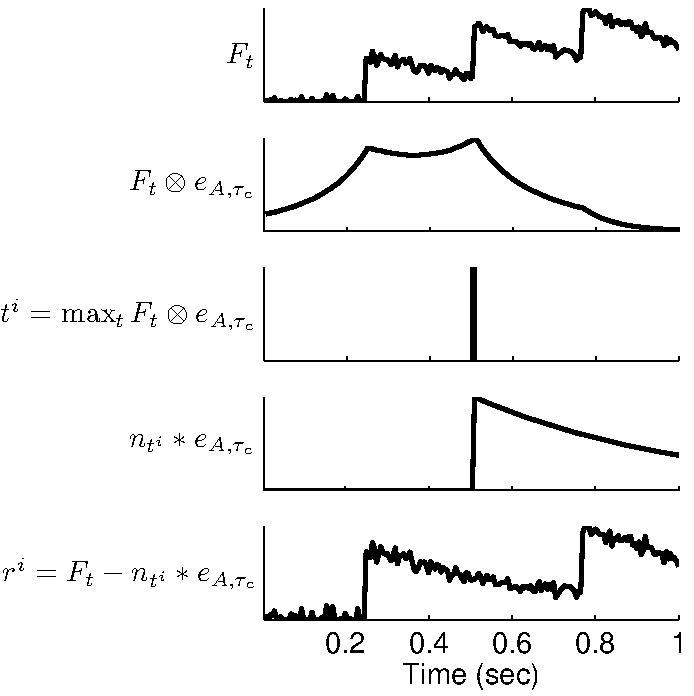
\includegraphics[height=0.8\textheight]{ppr_schem} 
\end{figure}


\newpage
\bibliography{C:/D/misc/biblist}
\addcontentsline{toc}{section}{References}
%\bibliographystyle{apalike}
\bibliographystyle{biophysj}



\end{document}
